% !TEX TS-program = pdflatexmk
% Template file for TeXShop by Michael Sharpe, LPPL
\documentclass[]{article}
\usepackage[margin=1in]{geometry} 
\usepackage[parfill]{parskip}% Begin paragraphs with an empty line rather than an indent
\usepackage{trace}
\usepackage{graphicx}
%\usepackage{amssymb}% don't use with newtxmath
%SetFonts
% libertine+newtxmath
\pdfmapfile{+NotoMath.map}
\usepackage[T1]{fontenc}
%\usepackage[scaled=1.1]{zlmtt}
%\usepackage[scaled=1.1]{newtxtt}
\usepackage[scaled=1.12]{nimbusmononarrow}
\usepackage[sfdefault,vvarbb]{notomath}
%\usepackage{noto-serif} 
%\usepackage{noto-sans} 
%\usepackage{noto-mono} 
%\usepackage{textcomp}
%%\usepackage[varqu,varl]{zi4}% inconsolata
%%\usepackage{amsmath,amsthm}
%\usepackage[noto,vvarbb]{newtxmath}
% option vvarbb gives you stix blackboard bold
\usepackage{bm}
\usepackage{fonttable}
%SetFonts
\title{Notomath---LaTeX math support for the noto package}
\author{Michael Sharpe}
\date{\today}  % Activate to display a given date or no date

\begin{document}
\maketitle
%\traceon$D$\traceoff

This package provides math support for the Google font collection {\tt Noto}, a massive text font whose \LaTeX\ support has been available for several years using Bob Tennent's {\tt noto} package. The math support is based on {\tt newtxmath} but there are some wrinkles that make it desirable to craft a small package, {\tt notomath}, that can serve as a front end to simplify the business of lining up the text and math options, given that there are considerable size discrepancies between text and math at their natural sizes. 

For the {\tt noto} option to {\tt newtxmath}, the Roman and Greek alphabets in the latter were substituted by those in {\tt Noto} scaled down by $10$\% to an x-height of $482$, which is a close enough match to the symbols in {\tt newtxmath} for all practical purposes. 
%The support is handled by means of an option to {\tt newtxmath}, which would not normally warrant a separate package, but there are some unusual wrinkles in this case that might go unnoticed otherwise.

%\makeatletter
%\show\NotoSans@scale
%\makeatother
The Noto fonts comprise three different faces: {\tt NotoSerif}, {\tt NotoSans} and {\tt NotoSansMono}. Each face has its own {\tt.sty} file: {\tt noto-serif.sty}, {\tt noto-sans.sty} and {\tt noto-mono.sty}. There is also an integrated {\tt.sty} file, {\tt noto.sty}, though it is a bit less configurable. Most of the time, it should not be necessary to load any of these packages explicitly, that task being relegated to the package {\tt notomath}.


\section*{Usage}
For most users, it will likely suffice to place some small variant of the following line in the preamble:
\begin{verbatim}
\usepackage{notomath}
\end{verbatim}
The effect of this is:
\begin{itemize}
\item
load {\tt noto-serif} and {\tt noto-sans} scaled down by the factor .9 to an x-height of 482;
\item set the main text font to NotoSerif and set \verb|\sfdefault| to 
NotoSans;
\item the only weight used from the nine available weights are {\tt regular} and {\tt bold}, as these are the weights used in {\tt newtxmath} with options {\tt noto} and {\tt notosans};
\item load {\tt newtxmath} with option {noto} at natural scale.
\end{itemize}

Alternatively, the package may be loaded with options that modify the above behaviors:
\begin{itemize}
\item {\tt mono} loads, in addition, {\tt noto-mono} at the same x-height as the other Noto text packages.
\item
{\tt scale} (or {\tt scaled}) allows you to rescale all the Noto text packages and newtxmath by the specified factor.
\item the figure style for NotoSerif and NotoSans may be controlled by the options {\tt proportional} (or {\tt pf}) and {\tt oldstyle} (or {\tt osf}), as in the {\tt noto} package. (The default setting is tabular, lining figures.)
\item You may add as an option to {\tt notomath} any  newtxmath option that is relevant to {\tt noto}---these are simply passed along to {\tt newtxmath}, if truly relevant. (E.g., option {\tt vvarbb} would be passed along, but not {\tt garamondx} because that would change all the math italic alphabets to match garamondx.)
\item {\tt sfdefault} changes the main text font to NotoSans, but leaves the meaning of \verb|\rmdefault| unchanged, so that \verb|\textrm{}| prints its argument using NotoSerif.

\end{itemize}

\section*{Usage Notes}
\begin{itemize}
\item
 There are a couple of issues that might lead you to avoid NotoSansMono as your Typewriter font:
\begin{itemize}
\item
In {\tt OT1} encoding, the glyphs are not laid out as {\tt TEX TYPEWRITER TEXT}, as, for example, {\tt cmtt}. This means you will get incorrect output from text that involves quotes, backslash, braces and the like.  (This is not a problem in other encodings such as {\tt T1}.)
\item The {\tt NotoSansMono} fonts have no {\tt visiblespace} glyph, so \verb|\verb*| will fail to to render the space as something like {\usefont{OT1}{cmtt}{m}{n}\char"20}. If this is important to you, replace {\tt noto-mono} with a package like {\tt inconsolata}, if you want to try another sans mono font. The loading order is important---you should load {\tt inconsolata} before loading {\tt notomath}.
\end{itemize}

\item
If you chose the {\tt sfdefault} option so that NotoSans is the main text font, you may find that a SansMono font if too similar to be easily distinguished from the main font, in which case you may wish to switch to a serifed mono font. If not loading NotoSansMono by means of the option {\tt mono}, you should load a replacement TT package BEFORE loading {\tt notomath} if you wish to be able to use the macro \verb|\mathtt| using glyphs that match those used for \verb|\texttt|. There are three reasonable options, and possibly more that I'm not aware of. Each would need to be scaled up a bit.
\begin{itemize}

\item The TT package {\tt zlmtt} does have a {\tt visiblespace} glyph and its {\tt OT1} encoding is in {\tt TEX TYPEWRITER TEXT} so \verb|\verb| and \verb|\texttt| function correctly even in {\tt OT1} encoding.  I find the caps too tall to be a very good match.
\item The TT package {\tt newtxtt} does have a {\tt visiblespace} glyph
and works well in {\tt T1} encoding. There is no {\tt OT1} encoded version currently. Caps are a bit too tall to be a very good match.
\item The TT package {\tt nimbusmononarrow} does have a {\tt visiblespace} glyph and its {\tt OT1} encoding is in {\tt TEX TYPEWRITER TEXT} so \verb|\verb| and \verb|\texttt| function correctly even in {\tt OT1} encoding. Caps are not too tall---this is my preferred serifed TT with NotoSans text.
\end{itemize}

\item 
\end{itemize}

 
\section*{Example preamble fragments}
\textsc{Example 1:}
\begin{verbatim}
\usepackage[mono,vvarbb,upint]{notomath} 
% load NotoSerif, NotoSans, NotoSansMono, mainfont=NotoSerif
% options vvarbb and upint passed to newtxmath, resulting in
% STIX Blackboard Bold and upright integrals rather than slanted
\end{verbatim}
The Noto fonts will be scaled to x-height 482, matching math symbols. The main text font will be NotoSerif.

\textsc{Example 2:}
\begin{verbatim}
\usepackage[varq,varl]{inconsolata} % inconsolata sans mono
\usepackage[vvarbb,uprightscript]{notomath} 
% load NotoSerif, NotoSans, mainfont=NotoSerif
% options vvarbb and uprightscript passed to newtxmath, resulting in
% STIX Blackboard Bold and upright script
\end{verbatim}
The Noto fonts will be scaled to x-height 482, matching math symbols. The main text font will be NotoSerif.

\textsc{Example 3:}
\begin{verbatim}
\usepackage[scaled=1.12]{nimbusmononarrow}% typewriter font
\usepackage[sfdefault,subscriptcorrection]{notomath}
% load NotoSerif, NotoSans, mainfont=NotoSans
% option subscriptcorrection passed to newtxmath
\end{verbatim}
will output the Noto fonts scaled to x-height 482 with matching math symbols. The main text font will be NotoSans.

\textsc{Example 4:}
\begin{verbatim}
\usepackage[scaled=1.24]{nimbusmononarrow}% typewriter font
\usepackage[scale=1.11,sfdefault,pf,osf]{notomath}
% load NotoSerif, NotoSans, mainfont=NotoSans
% option subscriptcorrection passed to newtxmath
\end{verbatim}
will output the Noto fonts scaled to x-height $536$ with matching math symbols. The main text font will be NotoSans with proportional oldstyle figures except in math, which always uses tabular lining figures.

The examples above all work with {\tt pdflatex}, and with {\tt xelatex} if some additional rules are followed. With {\tt xelatex}, the lines in the above examples must precede  the loading of {\tt fontspec}, which must use the option {\tt nomath}. After that, one may load any text fonts required for secondary use, or even replace the main Noto fonts.
\section*{Subscript Correction}
The spacing of math letters was adjusted so the superscripts would not collide with the base letters. This was necessary mainly for letters like $j$, $f$, $y$ and $\beta$ as superscripts and like $D$ and $\Omega$ as base letters. As a result of these adjustments, some of the formerly problematic superscript letters become problematic subscript letters. Two files are provided to make adjustments to the letter by inserting appropriate kerns when that letter is the first character in a subscript---one for NotoSerif and one for NotoSans letters, under the respective names 
\begin{verbatim}
newtx-noto-subs.tex % for NotoSerif
newtx-notosans-subs.tex
\end{verbatim}
The appropriate file is read in by {\tt newtxmath} provided you add the option {\tt subscriptcorrection}. A line in the file of the form \verb|{j}{-2}| will translate to a kern of {\tt -2mu} being placed before a leading $j$ in a subscript. 

\section*{Lower level settings}
It may be that you wish to make use of lower level settings in the individual {\tt noto-} packages. In that case, the following information may be useful.




Recall from the README to the {\tt noto}:
\begin{itemize}
\item
\verb|\usepackage{noto}|
   \begin{itemize}
   \item loads NotoSerif as \verb|\rmdefault|;
   \item loads NotoSans as \verb|\sfdefault|;
  \item loads NotoSansMono as \verb|\ttdefault|;
   \item lets \verb|\familydefault| to \verb|\rmdefault|;
   \item so, main body text is NotoSerif, \verb|\textsf| points to NotoSans and \verb|\texttt| to NotoSansMono. 
   \item The {\tt scale} option does not affect NotoSerif size.
   \end{itemize}
\item
\verb|\usepackage{noto-serif}|
   \begin{itemize}
   \item loads NotoSerif as \verb|\rmdefault|;
   \item lets \verb|\familydefault| to \verb|\rmdefault|;
   \item neither NotoSans nor NotoSansMono is loaded.
   \item {\tt scale} option available.
   \end{itemize}
\item
\verb|\usepackage{noto-sans}|
   \begin{itemize}
   \item loads NotoSans as \verb|\sfdefault|;
   \item does not modify \verb|\familydefault|;
   \item neither NotoSerif or NotoSansMono is loaded.
   \item {\tt scale} option available.
\end{itemize}
\item
\verb|\usepackage[sfdefault]{noto-sans}| 
   \begin{itemize}
   \item loads NotoSans as \verb|\sfdefault|;
   \item lets \verb|\familydefault| to \verb|\sfdefault|
   \item neither NotoSerif or NotoSansMono is loaded and NotoSans becomes the main text font.
      \item {\tt scale} option available.
\end{itemize}
\item
\verb|\usepackage{noto-mono}|
   \begin{itemize}
   \item loads NotoSansMono as \verb|\ttdefault|;
   \item neither NotoSerif or NotoSans is loaded.   
      \item {\tt scale} option available.
\end{itemize}
\end{itemize}

At its lowest level, you invoke NotoMath in {\tt newtxmath} using the option {\tt noto}, and NotoSansMath using the option  {\tt notosans}.

\section*{Math samples}
\def\bE{\mathbf{E}}
\def\bB{\mathbf{B}}
\def\bJ{\mathbf{J}}

\def\bx{\mathbf{x}}
\def\by{\mathbf{y}}
\def\bv{\mathbf{v}}
\def\bp{\mathbf{p}}
\def\bxdot{\mathbf{\dot x}}
\def\bal{\boldsymbol{\alpha}}
\def\bphi{\boldsymbol{\varphi}}
\def\e{\varepsilon}
\textbf{An inversion formula:} Let $g:\mathbb{R}^+\to \mathbb{R}$
 be bounded and right continuous, and let
$\varphi(\alpha)\coloneq\int_0^\infty e^{-\alpha t}g(t)\,dt$ denote its Laplace transform. Then, for every $t>0$,
\begin{equation}
g(t)=\lim_{\mathstrut\e\to 0}\lim_{\mathstrut\lambda\to\infty}\e^{-1}\sum_{\lambda t<k\le (\lambda+\e)t}
\frac{(-1)^k}{k!}\lambda^k\varphi ^{(k)}(\lambda).
\end{equation}

\textbf{Solutions of systems of ODEs:} Let $\bv(\bx,\bal)$ denote a parametrized vector field ($\bx\in U$, $\bal\in A$) where $U$ is a domain in $\mathbb{R}^n$ and the parameter space $A$ is a domain in $\mathbb{R}^m$. We assume that $\bv$ is $C^k$-differentiable as a function of~$(\bx,\bal)$, where~$k\ge 2$. Consider a system of differential equations in~$U$:
\begin{equation}
\bxdot=\bv(\bx,\bal),\qquad \bx\in U\label{eq:first}
\end{equation}
 Fix an initial point $\bp_0$ in the interior of $U$, and assume $\bv(\bp_0,\bal_0)\neq\mathbf{0}$. Then, for sufficiently small $t$, $|\bp-\bp_0|$ and $|\bal-\bal_0|$, the system~(\ref{eq:first}) has a unique solution $\bx_{\bal}(t)$  satisfying the initial condition $\bx_{\bal}(0)=\bp$, and that solution depends differentiably (of class~$C^k$) on $t$, $\bp$ and $\bal$.

\textbf{Stirling's formula:} 
\begin{equation}
\Gamma(z)\sim e^{-z}z^{z-1/2}\sqrt{2\pi}\bigg[1+\frac{1}{12z}+\frac{1}{288z^2}-\frac{139}{51840z^3}+\ldots\bigg],\quad z\to\infty \text{ in $|\arg z|<\pi$}.
\end{equation}

\textbf{B\'ezier curves:} Given $z_1$,
$z_2$,
$z_3$,
$z_4$ in  $\mathbb{C}$, define  the B\'ezier
curve with control points $z_1$, $z_2$, $z_3$, $z_4$ by
\[z(t)\coloneq(1-t)^3z_1+3(1-t)^2tz_2+3(1-t)t^2z_3+t^3z_4,\qquad 0\le t\le 1.\]
Because $(1-t)^3+3(1-t)^2t+3(1-t)t^2+t^3=(1-t+t)^3=1$
and all summands are positive for $0\le t\le1$, $z(t)$
is a convex combination of the four points~$z_k$, hence
the curve defined by $z(t)$ lies in their convex hull. As $t$ varies from~$0$ to~$1$, the curve moves from
$z_1$ to~$z_4$ with initial direction $z_2-z_1$ and final direction $z_4-z_3$. 

\textbf{Maxwell's equations:}
\begin{equation*}
\begin{aligned}
\bB'&=-c\nabla\times\bE\\
\bE'&=c\nabla\times\bB-4\pi \bJ.
\end{aligned}
\end{equation*}

\textbf{Residue theorem:} Let $f$ be analytic in the region $G$ except for the isolated singularities $a_1$, $a_2$, \ldots, $a_m$. If $\gamma$ is a closed rectifiable curve in $G$ which does not pass through any of the points $a_k$ and if $\gamma\approx 0$ in $G$, then
\[\frac{1}{2\pi i}\int_\gamma f=\sum_{k=1}^m n(\gamma;a_k)\,\mathrm{Res}(f;a_k).\]

\textbf{Maximum modulus principle:} Let $G$ be a bounded open set in  $\mathbb{C}$ and suppose that $f$ is a continuous function on $\bar G$ which is analytic in $G$. Then
\[\max \{|f(z)| : z\in \bar G\}=\max\{|f(z)| : z\in \partial G\}.\]

\textbf{Jacobi's identity:} Define the \emph{theta function}  $\vartheta$ by
\[\vartheta(t)=\sum_{n=-\infty}^\infty \exp(-\pi n^2 t),\qquad t>0.\]
 Then
\[\vartheta(t)=t^{-1/2}\vartheta(1/t).\]

The following three samples show the previous three reworked using NotoSerif and its associated math fonts.

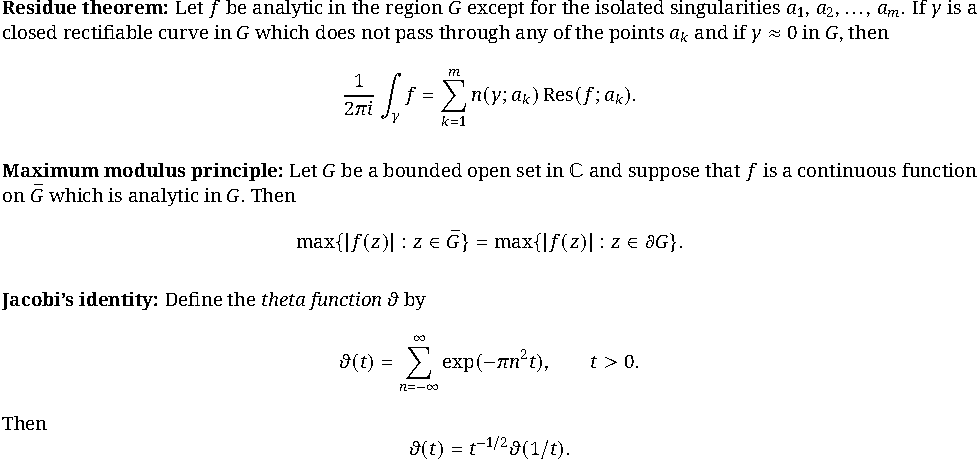
\includegraphics{samplerSerif-crop.pdf}
\newpage
\section*{Font Tables}
\textsc{Sans Math Letters}
\fonttable{notosansmi}

\newpage

\textsc{Sans Math LettersA}
\fonttable{notosansmia}

\newpage
\textsc{Serif Math Letters}
\fonttable{notomi}

\newpage

\textsc{Serif Math LettersA}
\fonttable{notomia}
%\setbox0\hbox{\textrm{x}}
%\showthe\ht0
\end{document}  